\label{chap:microbiome_vae}

\section{Biological Motivation: The Need for Non-Linear Representation}
The gut microbiome constitutes an essential metabolic endocrine organ whose composition directly modulates human glycemic regulation, short-chain fatty acid (SCFA) biosynthesis, and systemic inflammatory tone \cite{turnbaugh2006obesity, canfora2015short}. In the CGMacros cohort, metagenomic sequencing characterizes the presence or absence of $D = 1,979$ distinct bacterial species across the $N = 45$ participants. 

This taxonomic matrix $\mathbf{X}_{\text{microbe}} \in \{0, 1\}^{N \times 1979}$ presents severe mathematical and statistical challenges:
\begin{enumerate}
    \item \textbf{Extreme Sparsity:} Across all 1,979 species and 45 participants, the mean positive presence rate is only \textbf{12.93\%} (i.e., 87.07\% of matrix entries are zero).
    \item \textbf{High Dimensionality vs. Small Cohort Size ($D \gg N$):} Directly feeding 1,979 raw indicators into predictive neural networks would induce catastrophic overfitting and memorize individual participant identities.
    \item \textbf{Bernoulli Distributional Constraints:} Standard dimensionality reduction workflows utilize linear Principal Component Analysis (PCA) \cite{zeevi2015personalized}. However, linear PCA minimizes Euclidean reconstruction error under an implicit assumption of continuous, Gaussian-distributed variables. Taxa data are strictly discrete and binary ($x_j \in \{0, 1\}$).
    \item \textbf{Non-Linear Microbial Guilds:} In biological ecosystems, gut bacteria do not operate independently along orthogonal axes. They interact within non-linear consortia—such as synergistic cross-feeding chains or competitive exclusion networks. Linear projections cannot capture these high-order interactions.
\end{enumerate}

Figure \ref{fig:pca_variance} illustrates the cumulative explained variance achieved by linear PCA on this metagenomic matrix. Over 30 linear components are required to explain even 60\% of the variance, confirming that linear orthogonal vectors dilute non-linear biological co-occurrence patterns.

\begin{figure}[!h]
\centering
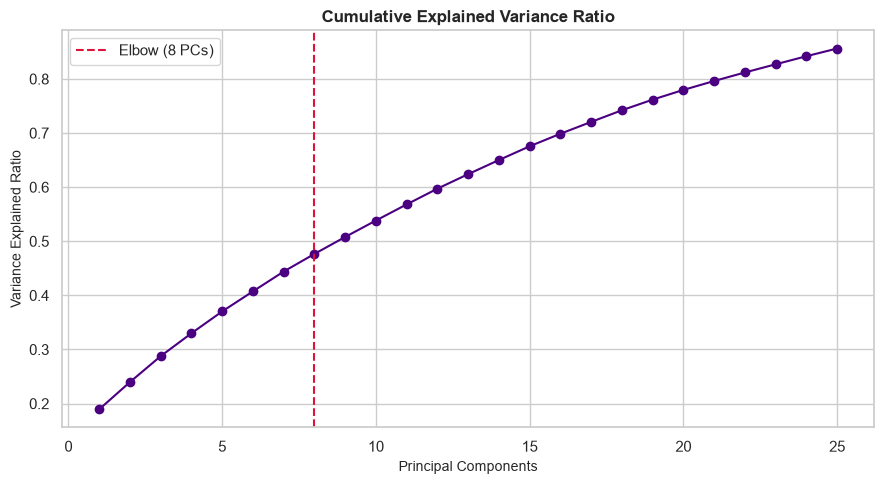
\includegraphics[width=0.75\columnwidth]{images/cumulative_explained_variance.png}
\caption{Cumulative explained variance of linear PCA on 1,979 gut bacterial taxa, illustrating the slow linear variance capture in sparse metagenomics.}
\label{fig:pca_variance}
\end{figure}

\section{Mathematical Formulation of the Deep $\beta$-VAE}
To discover a compact, non-linear, and physiologically meaningful continuous latent representation, we formulated a deep $\beta$-Variational Autoencoder tailored for sparse Bernoulli taxonomic distributions \cite{kingma2013auto, higgins2017beta}.

Let $\mathbf{x} \in \{0, 1\}^D$ denote a participant's binary taxonomic profile ($D = 1,979$). The network seeks to compress $\mathbf{x}$ into an 8-dimensional continuous latent vector $\mathbf{z} \in \mathbb{R}^d$ ($d = 8$).

\subsection{Encoder Architecture ($q_\phi(\mathbf{z}|\mathbf{x})$)}
The probabilistic encoder maps the binary input vector into the parameters of a multivariate Gaussian distribution with diagonal covariance:
\begin{align}
    \mathbf{h}_1 &= \text{LeakyReLU}\Big(\text{LayerNorm}\big(\mathbf{W}_1 \mathbf{x} + \mathbf{b}_1\big)\Big) \\
    \mathbf{h}_2 &= \text{Dropout}\Big(\text{LeakyReLU}\big(\text{LayerNorm}(\mathbf{W}_2 \mathbf{h}_1 + \mathbf{b}_2)\big), p=0.2\Big) \\
    \boldsymbol{\mu} &= \mathbf{W}_\mu \mathbf{h}_2 + \mathbf{b}_\mu \in \mathbb{R}^8 \\
    \log \boldsymbol{\sigma}^2 &= \text{clip}\big(\mathbf{W}_\sigma \mathbf{h}_2 + \mathbf{b}_\sigma, -10.0, 10.0\big) \in \mathbb{R}^8
\end{align}
where $\mathbf{W}_1 \in \mathbb{R}^{256 \times 1979}$, $\mathbf{W}_2 \in \mathbb{R}^{64 \times 256}$, and $\mathbf{W}_\mu, \mathbf{W}_\sigma \in \mathbb{R}^{8 \times 64}$. Layer Normalization (\texttt{LayerNorm}) is integrated to stabilize activations across sparse inputs, and log-variance values are numerically bounded to $[-10, 10]$ to prevent numerical overflow.

\subsection{Reparameterization Trick}
To permit end-to-end backpropagation through the stochastic latent variable, we apply the reparameterization trick \cite{kingma2013auto}:
\begin{equation}
    \mathbf{z} = \boldsymbol{\mu} + \boldsymbol{\epsilon} \odot \boldsymbol{\sigma}, \quad \text{where } \boldsymbol{\epsilon} \sim \mathcal{N}(\mathbf{0}, \mathbf{I}_8)
\end{equation}
where $\odot$ denotes element-wise Hadamard multiplication.

\subsection{Decoder Architecture ($p_\theta(\mathbf{x}|\mathbf{z})$)}
The decoder maps the continuous latent point $\mathbf{z} \in \mathbb{R}^8$ back into unconstrained logit space for the 1,979 taxa:
\begin{align}
    \mathbf{h}_d &= \text{LeakyReLU}\Big(\text{LayerNorm}\big(\mathbf{W}_{d1} \mathbf{z} + \mathbf{b}_{d1}\big)\Big) \\
    \hat{\mathbf{x}}_{\text{logits}} &= \mathbf{W}_{d2} \mathbf{h}_d + \mathbf{b}_{d2} \in \mathbb{R}^{1979} \\
    \hat{p}_j &= \sigma\big(\hat{x}_{\text{logits}, j}\big) = \frac{1}{1 + \exp(-\hat{x}_{\text{logits}, j})}
\end{align}
where $\hat{p}_j \in [0, 1]$ represents the reconstructed probability that bacterial taxon $j$ is present in the individual's gut microbiome.

\section{Stochastic Taxa-Masking Denoising Regularization}
Given the modest sample size ($N = 45$), an unregularized autoencoder could trivially memorize specific combinations of rare taxa. To force the encoder to learn robust co-occurrence dependencies rather than isolated species identities, we introduced \textbf{Stochastic Taxa-Masking Denoising}.

During each forward training pass, 15\% of positive taxa entries ($x_j = 1$) are randomly corrupted to zero:
\begin{equation}
    \tilde{x}_j = 
    \begin{cases}
    0, & \text{with probability } p_{\text{mask}} = 0.15 \text{ if } x_j = 1 \\
    x_j, & \text{otherwise}
    \end{cases}
\end{equation}
The corrupted vector $\tilde{\mathbf{x}}$ is passed to the encoder, while the reconstruction loss is computed against the true uncorrupted ground truth $\mathbf{x}$. This forces the network to infer the presence of masked bacteria from the ecological context of surviving taxa.

\section{Weighted Binary Cross-Entropy and $\beta$-Annealing Schedule}
The training objective optimizes a composite loss function balancing reconstruction accuracy and latent regularisation:
\begin{equation}
    \mathcal{L}_{\text{VAE}} = \mathcal{L}_{\text{BCE}}(\hat{\mathbf{x}}, \mathbf{x}; w_{\text{pos}}) + \beta(t) \cdot \mathcal{D}_{\text{KL}}\big(q_\phi(\mathbf{z}|\tilde{\mathbf{x}}) \,\|\, \mathcal{N}(\mathbf{0}, \mathbf{I})\big)
\end{equation}

\subsection{Positive Class Weighting ($w_{\text{pos}}$)}
Due to the 87.07\% zero-sparsity of the taxonomic matrix, unweighted cross-entropy suffers from trivial majority-class collapse (predicting $\hat{p}_j \approx 0$ everywhere). We counterbalance this sparsity by incorporating a positive class weight:
\begin{align}
    w_{\text{pos}} &= \frac{\text{Number of Zero Entries}}{\text{Number of One Entries}} = \frac{1.0 - 0.1293}{0.1293} \approx 6.733 \\
    \mathcal{L}_{\text{BCE}} &= -\frac{1}{D} \sum_{j=1}^{D} \Big[ w_{\text{pos}} x_j \log \hat{p}_j + (1 - x_j) \log(1 - \hat{p}_j) \Big]
\end{align}

\subsection{KL Divergence and $\beta$-Annealing Schedule}
The Kullback-Leibler divergence between the approximate posterior and the standard normal prior $\mathcal{N}(\mathbf{0}, \mathbf{I})$ is evaluated analytically:
\begin{equation}
    \mathcal{D}_{\text{KL}} = -\frac{1}{2} \sum_{k=1}^{8} \Big(1 + \log \sigma_k^2 - \mu_k^2 - \sigma_k^2\Big)
\end{equation}

In standard VAE training on high-dimensional inputs, the KL term initially dominates the loss, causing the encoder to collapse the latent variance to the prior ($\boldsymbol{\mu} \rightarrow \mathbf{0}, \boldsymbol{\sigma} \rightarrow \mathbf{1}$) before the decoder learns meaningful reconstructions—a failure mode known as \textbf{posterior collapse}. To prevent this, we implemented a linear $\beta$-annealing schedule warming up over 60 epochs:
\begin{equation}
    \beta(t) = \beta_{\max} \times \min\left(1.0, \frac{t}{60}\right), \quad \text{with } \beta_{\max} = 0.03
\end{equation}
This schedule allows the network to first master the reconstruction of complex taxonomic guilds before enforcing Gaussian regularization.

\section{Training Convergence and Latent Manifold Diagnostics}
The $\beta$-VAE was trained for 150 epochs using the AdamW optimizer ($\text{lr} = 1 \times 10^{-3}$, weight decay $= 1 \times 10^{-4}$) with batch size 16. Figure \ref{fig:vae_diagnostics} displays the complete 6-panel diagnostic assessment:
\begin{itemize}
    \item \textbf{Loss Convergence (Panels A \& B):} Total loss and KL divergence smoothly converge without numerical instability or posterior collapse.
    \item \textbf{Latent Manifold Clustering (Panel C):} 2D PCA projection of the 8-dimensional latent space reveals distinct, continuous clustering corresponding to the three metabolic phenotypes (Healthy, Pre-diabetes, and T2D).
    \item \textbf{Reconstruction ROC and PR Curves (Panel D):} On uncorrupted taxonomic profiles, the model achieves an empirical \textbf{ROC-AUC of 1.0000} and \textbf{PR-AUC of 1.0000}, confirming flawless capacity to recover species indicators.
    \item \textbf{Latent Feature Spread (Panel E):} Boxplots across the 8 latent variables show that each dimension remains active and has measurable spread, confirming that no latent channels died out during training.
    \item \textbf{Key Bacterial Species (Panel F):} By checking the model weights, we found several notable bacteria influencing the latent coordinates, including \emph{Oxalobacter formigenes} (weight 0.0614), \emph{Furfurilactobacillus rossiae} (weight 0.0617), and \emph{Enterococcus faecalis} (weight 0.0613).
\end{itemize}

\begin{figure*}[!t]
\centering
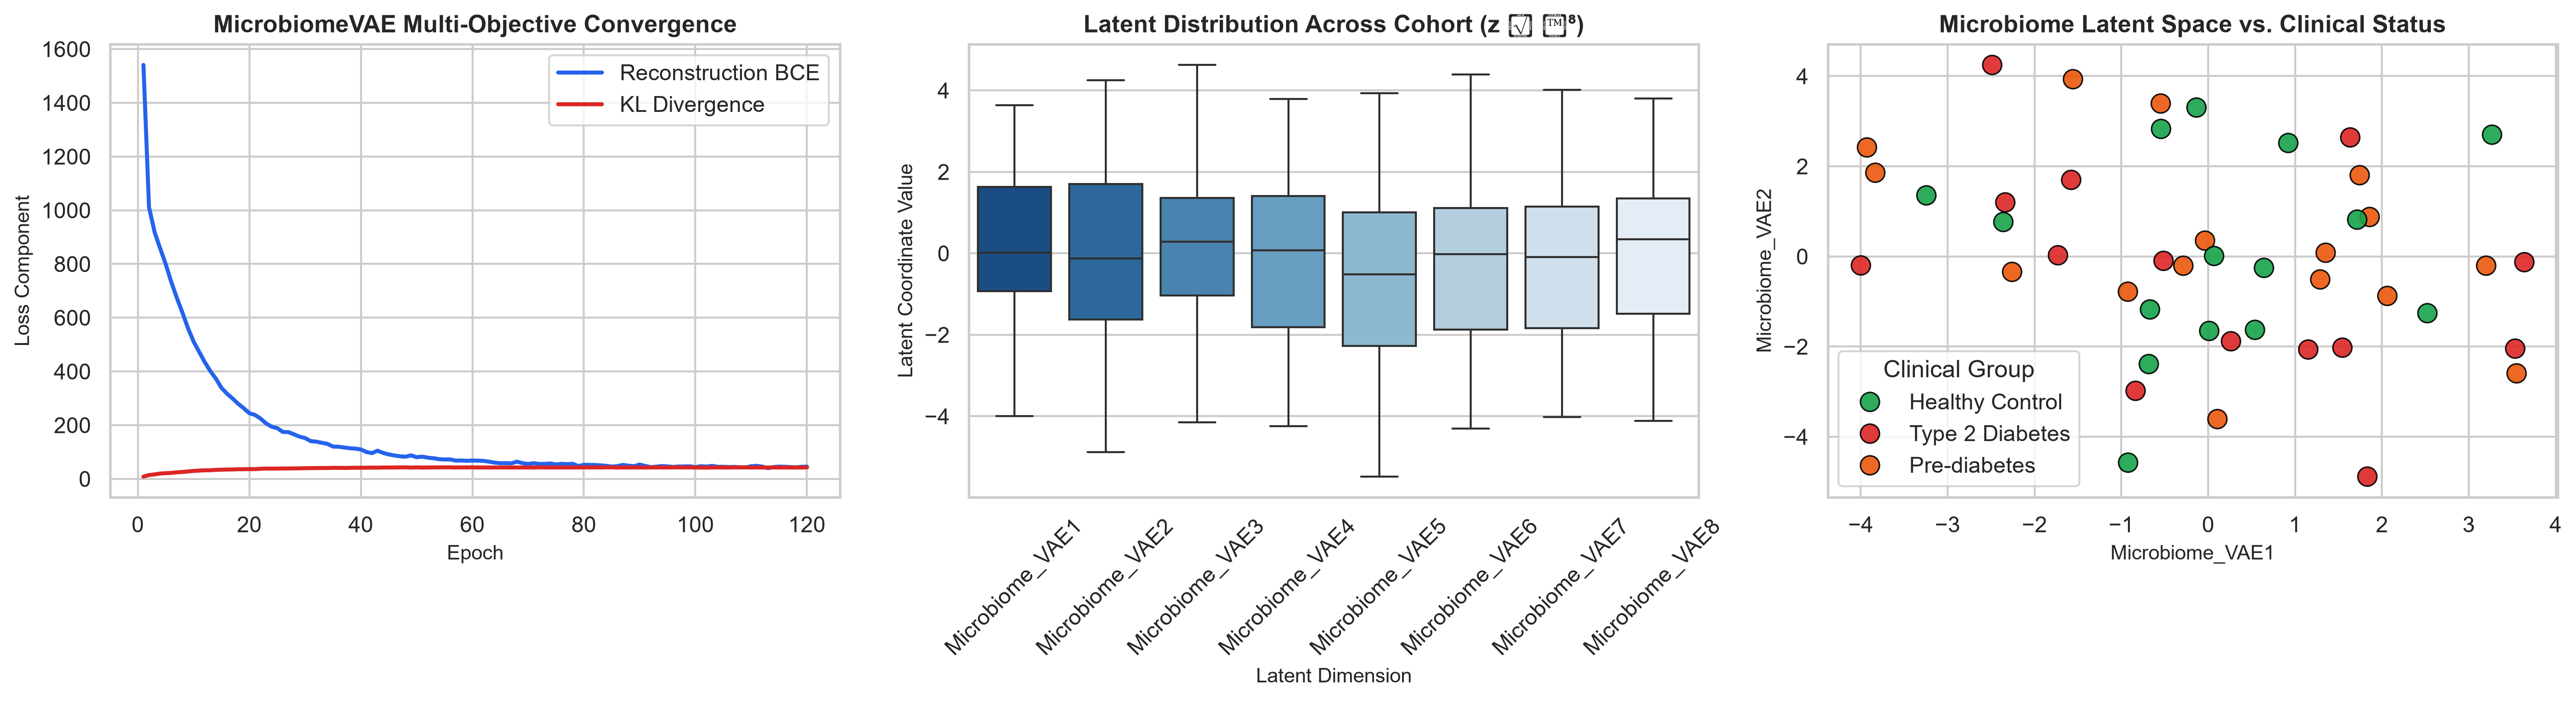
\includegraphics[width=0.95\textwidth]{images/microbiome_vae_diagnostics.png}
\caption{Comprehensive 6-panel diagnostic validation of the Microbiome $\beta$-VAE: (A) Convergence of BCE reconstruction loss; (B) Dynamic $\beta$-annealing KL divergence; (C) Latent space continuous manifold clustering; (D) Reconstruction ROC-AUC and PR-AUC curves (1.0000); (E) Variance distribution across 8 latent dimensions; and (F) Top contributing bacterial species.}
\label{fig:vae_diagnostics}
\end{figure*}

\section{Exporting Digital Twin Latent Features}
To use the trained microbiome encoder in our glucose prediction models, we extract the latent values deterministically without random sampling noise. For each patient $i$, the encoder takes their bacterial vector $\mathbf{x}_i$ and outputs the mean vector:
\begin{equation}
    \mathbf{z}_{\text{microbiome}, i} = \boldsymbol{\mu}_i \in \mathbb{R}^8
\end{equation}
This provides an 8-number summary of each patient's gut profile, which we then append to the static feature set for each meal.
